\section{Laboratory Lecture 2 BIS: 555 Timer}

\subsection{Introduction}

Up until this point we have seen how to manipulate clock signals by using frequency dividers, but what if we want to obtain a specific type of output response, for instance a single pulse or a clock with a duty cycle different from 50\% ? In this case, a multivibrator circuit is needed. \medskip

These type of integrated circuits use an RC timer to set the pulse duration and, depending on the manufacturer, they may work in different modes, i.e.:

\begin{enumerate}
    \item Clock generator circuits (Astable Multivibrator)
    
    \item One-Shot (Monostable Multivibrator)
    \begin{itemize}
        \item Retriggerable
        \item Non-Retriggerable
    \end{itemize}
\end{enumerate}

\subsubsection{Astable Multivibrator}

The first type of circuit, the \textbf{Astable Multivibrator}, is what is commonly referred to as \textbf{"Clock"}. These simple circuits basically switch back and forth between two unstable states with a specific duty cycle\footnote{The duty cycle of a digital circuit is the percentage of the ratio of pulse duration, or pulse width to the total period. It can be expressed as: 

\begin{equation*}
    D = \frac{t_{ON}}{t_{ON} + t_{OFF}} \cdot 100
    \label{fig:DUTY}
\end{equation*}
} set by an RC circuit. \medskip

In the previous section we have seen how modify a clock signal to obtain a specific output frequency, taking into account the limitations of an even division of course. The problem with this type of circuits is that they cannot provide custom duty cycles, which are needed in real case scenarios. That is when astable circuits come in handy.\medskip

\subsubsection{Monostable Multivibrator}

On the other hand, we can also find \textbf{Monostable Multivibrators}, commonly referred to as \textbf{"One-Shots"}. These type of circuits, as the name suggests, only output a single pulse when triggered, that is, they have only one stable state. The change from stable to quasi-stable occurs for a fixed time period $\mathbf{t_{p}}$ or $\mathbf{t_{w}}$ which is determined by an RC constant as well.\medskip

These circuits are readily available and they usually come in two forms, i.e. a retriggerable and a non-retriggerable one. When a retriggerable one-shot is triggered before the end of the pulse, the pulse duration $\mathbf{t_{p}}$, is restarted. Contrarily, when a non-retriggerable monostable is triggered before the end of the pulse, the output remains the same, in other words, the input is ignored until the output returns to the steady state.\medskip


\clearpage

We can visualise their behaviour in the following graphs:

\begin{figure}[H]
    \centering
    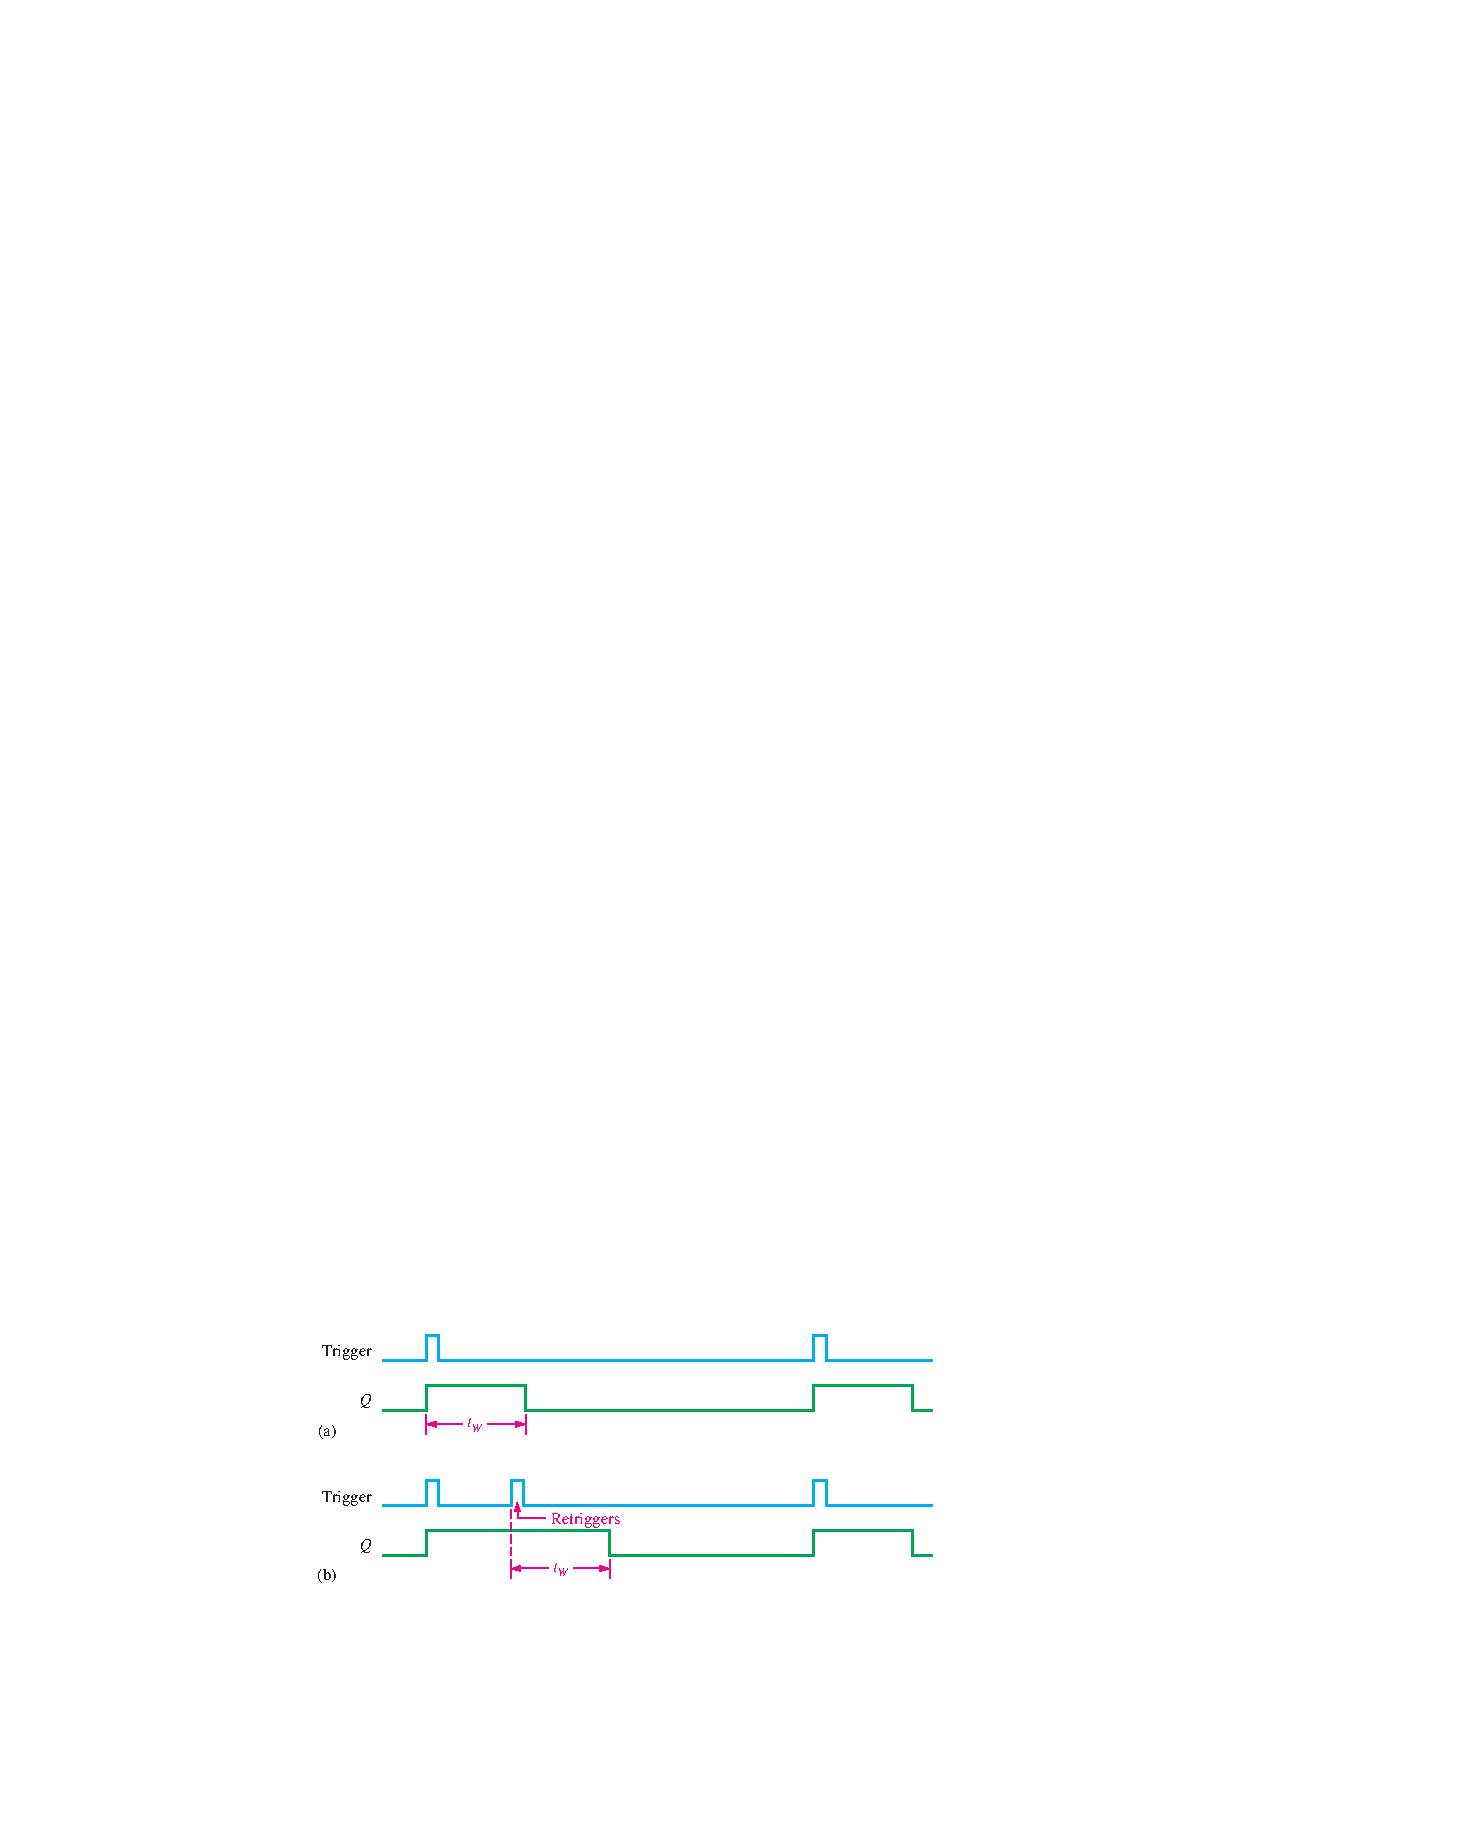
\includegraphics[scale = 1]{Graphics/Practice 2/GRAPHICS/MONOSTABLE/RETRIGGERABLE.pdf}
    \caption{Retriggerable Monostable. ~\autocite{FLOYD}}
    \label{fig:RETRIGGERABLE}
\end{figure}

\begin{figure}[H]
    \centering
    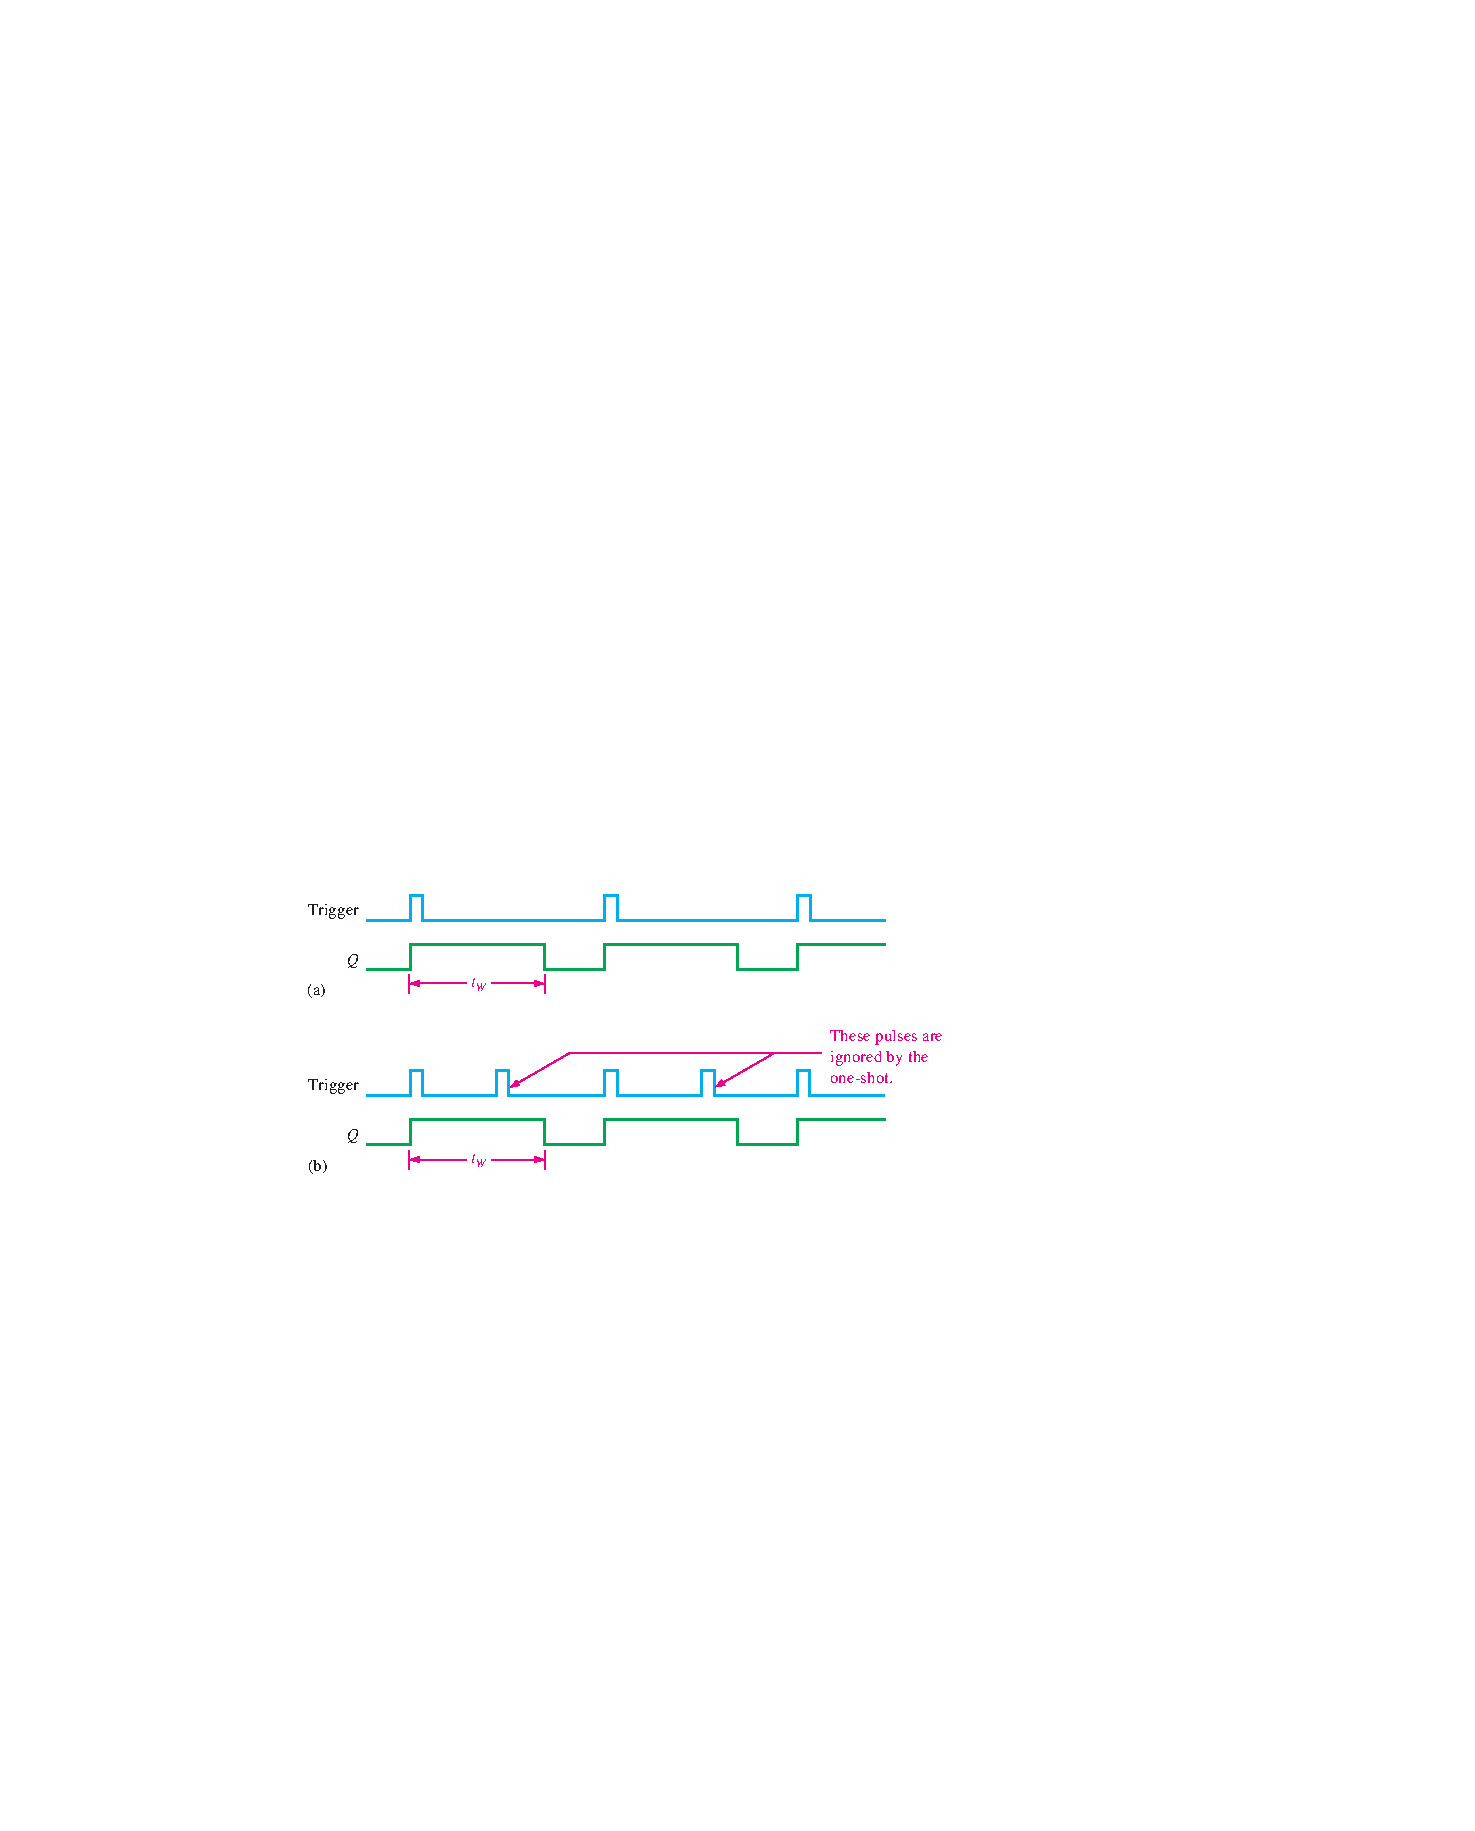
\includegraphics[scale = 1]{Graphics/Practice 2/GRAPHICS/MONOSTABLE/NON-RETRIGGERABLE.pdf}
    \caption{Non-Retriggerable Monostable. ~\autocite{FLOYD}}
    \label{fig:NON-RETRIGGERABLE}
\end{figure}


Both monostables, as well as the astable one, can be implemented using VHDL, but we will not dive into this, as it is not required in this practice, though they can be found \href{https://drive.google.com/open?id=1J-T80ZyF3isizOMjBf8xZOD7rw0KesP-}{\textbf{here}}.

\clearpage

\subsection{555 Timer}

Now that every type of multivibrator has been introduced, we will discuss the 555 timer. This timer is a TTL-compatible device that can operate in both of the modes described above. The heart of the 555 timer is composed of two voltage comparators and a SR Latch (See \ref{fig:SR_Asynch}). \medskip

The comparators are devices whose outputs are HIGH when the voltage on the positive (\texttt{+}) input is greater than the voltage on the negative (\texttt{-}) input and LOW when the (\texttt{-}) input voltage is greater than the (\texttt{+}) input voltage. \medskip

The voltage divider consisting of three 5 k$\Omega$ resistors provides a trigger level of $\frac{1}{3}$ VCC and a threshold level of $\frac{2}{3}$ VCC. The control voltage input (pin 5) can be used to externally adjust the trigger and threshold levels to other values if necessary.\medskip 

When the normally HIGH trigger input momentarily goes below $\frac{1}{3}$ VCC, the output of comparator B switches from LOW to HIGH and sets the S-R latch, causing the output (pin 3) to go HIGH and turning the discharge transistor Q1 off.\medskip

The output will stay HIGH until the normally LOW threshold input goes above $\frac{2}{3}$ VCC and
causes the output of comparator A to switch from LOW to HIGH. This resets the latch,
causing the output to go back LOW and turning the discharge transistor on. The external
reset input can be used to reset the latch independent of the threshold circuit. The trigger
and threshold inputs (pins 2 and 6) are controlled by external components connected to
produce either monostable or astable action. ~\autocite{FLOYD}


\begin{figure}[H]
    \centering
    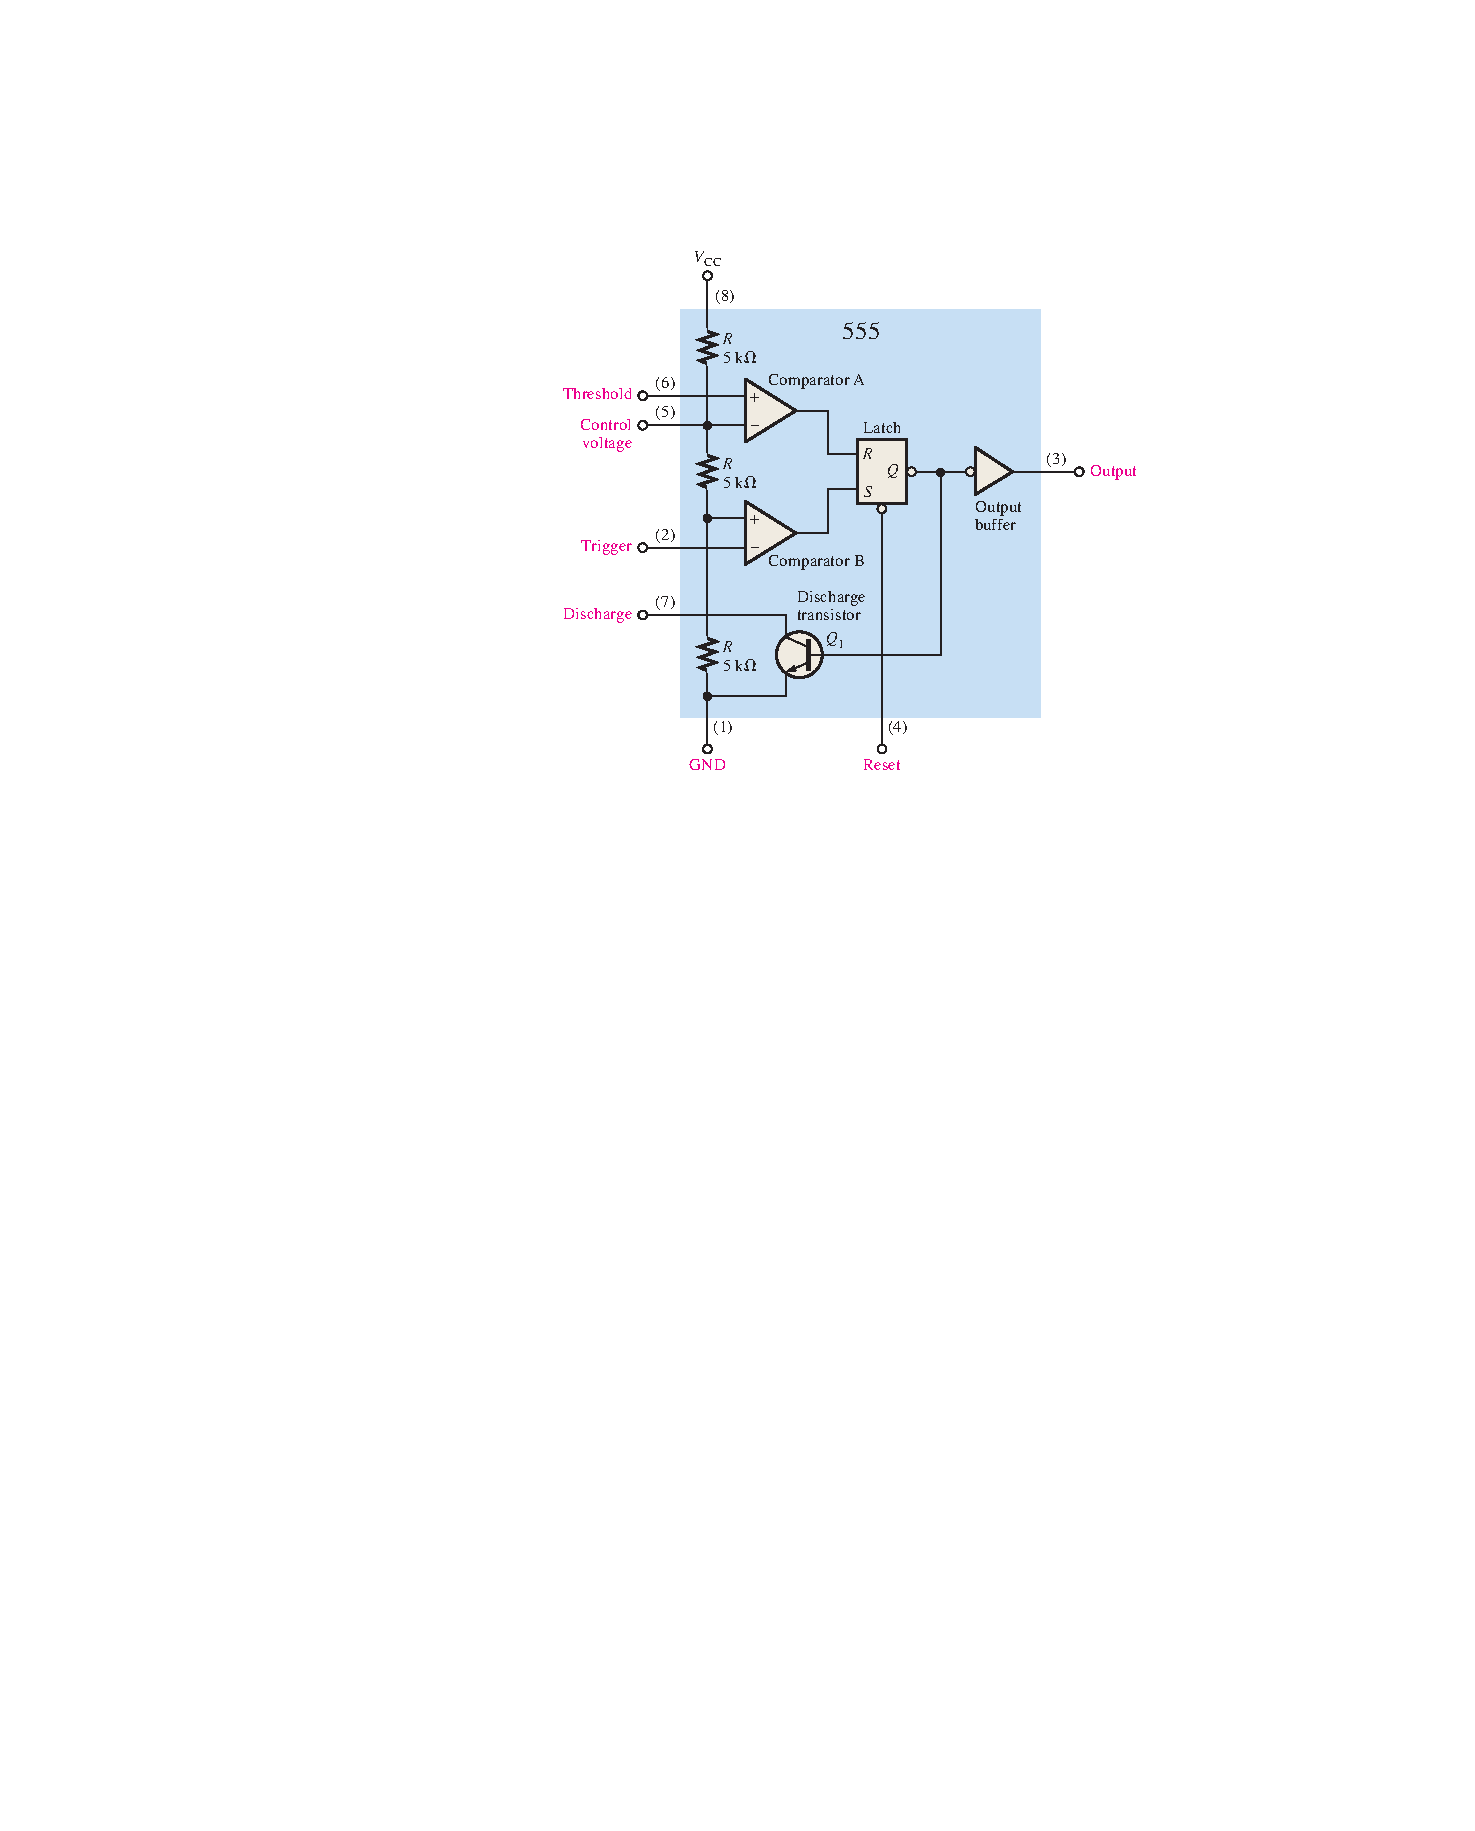
\includegraphics[scale = 0.99]{Graphics/Practice 2/GRAPHICS/555/GRAPHS/DATASHEETS/555_INTERNALS.pdf}
    \caption{Internal functional diagram of a 555 timer. ~\autocite{FLOYD}}
    \label{fig:555_DIAGRAM}
\end{figure}


\subsubsection{Astable 555}

As we have mentioned before, the 555 timer can be configured as a basic \textbf{Astable Multivibrator} following the circuit down below:

\begin{figure}[H]
    \centering
    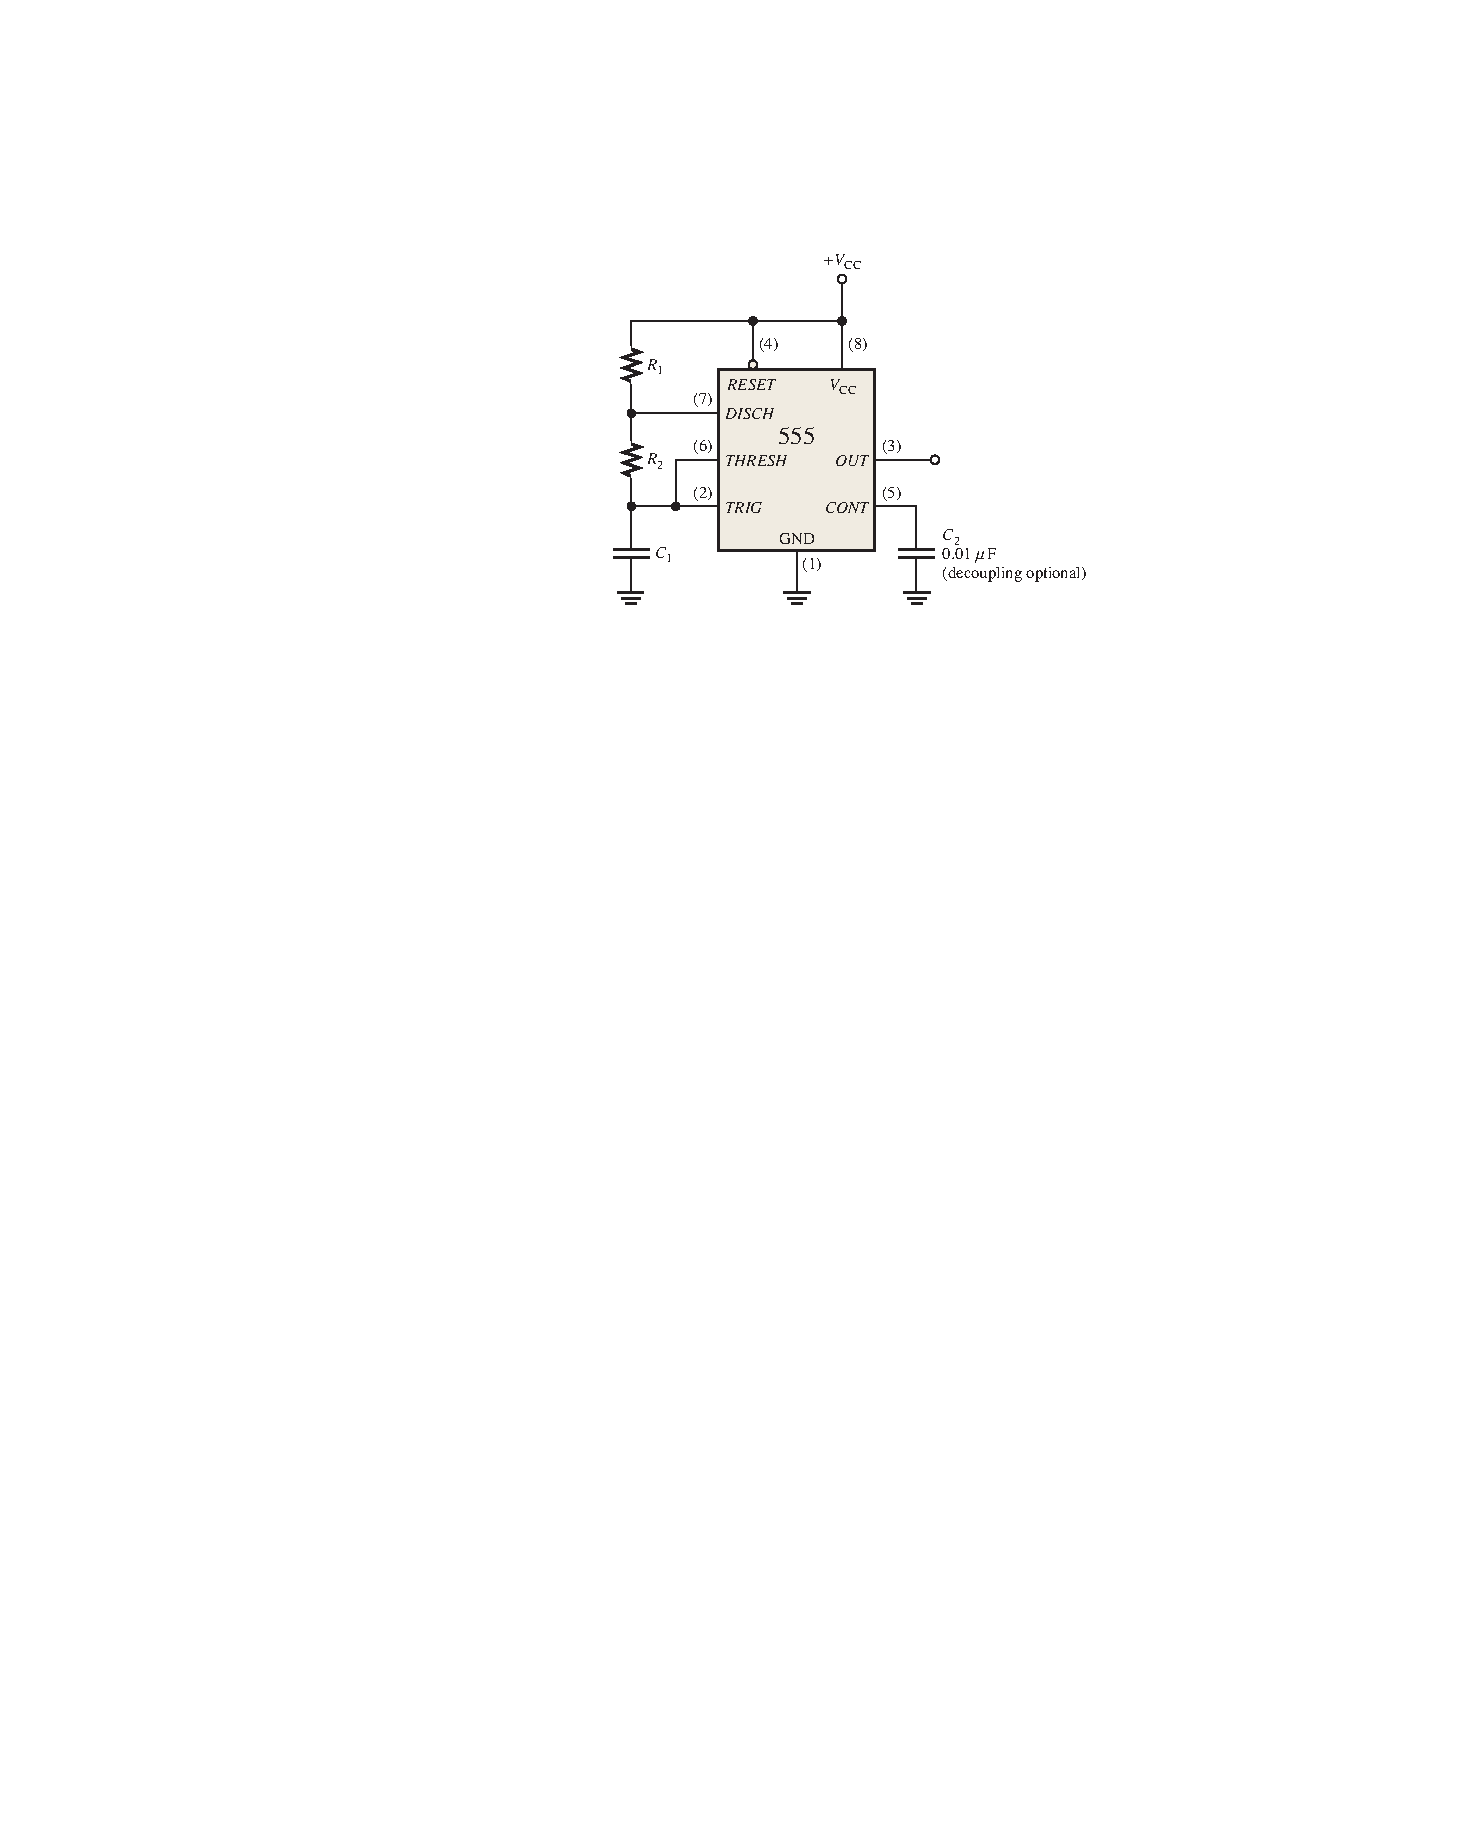
\includegraphics[scale = 1]{Graphics/Practice 2/GRAPHICS/555/GRAPHS/MODES/ASTABLE.pdf}
    \caption{555 timer connected as an astable multivibrator (oscillator). ~\autocite{FLOYD}}
    \label{fig:ASTABLE}
\end{figure}

In this circuit C1 charges through R1 and R2 and discharges through only R2. The output frequency is given by:

\begin{equation*}
    f = \frac{1.44}{(R_1 + 2\cdot R_2) \cdot C_1}
\end{equation*}

\vspace{0.25cm}

In order to help us find a set of suitable component values, the manufacturer provides a chart that shows sets of compatible and valid configurations. Besides, some useful equations are provided:

\vspace{0.6cm}

\begin{minipage}{\textwidth}
    \begin{minipage}[c]{0.49\textwidth}
        \centering
        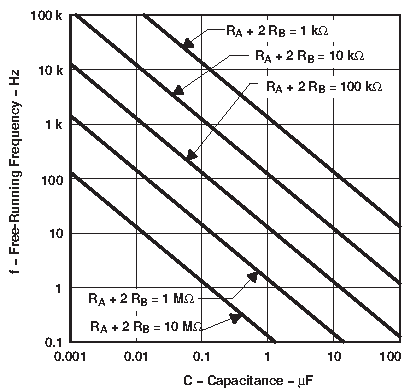
\includegraphics[scale=1]{Graphics/Practice 2/GRAPHICS/555/GRAPHS/DATASHEETS/ASTABLE_FREQ.pdf}
        \captionof{figure}{555 Astable Freq. Chart. ~\autocite{555_DS}}
        \label{fig:ASTABLE_FREQ}
    \end{minipage}
    \hfill
    \begin{minipage}[c]{0.49\textwidth}
        \centering
            \begin{align*}
                t_H &= 0.693 \cdot (R_1 + R_2) \cdot C_1& \\
                t_L &= 0.693 \cdot (R_2) \cdot C_1& \\
                T &= 0.693 \cdot (R_1 + 2\cdot R_2) \cdot C_1& \\
            \end{align*}
            
            \vspace{1.5cm}
    \end{minipage}
\end{minipage}

    
\subsubsection{Monostable 555}

The 555 timer can also be used as a \textbf{Monostable Multivibrator} following the circuit down below. 

\begin{figure}[H]
    \centering
    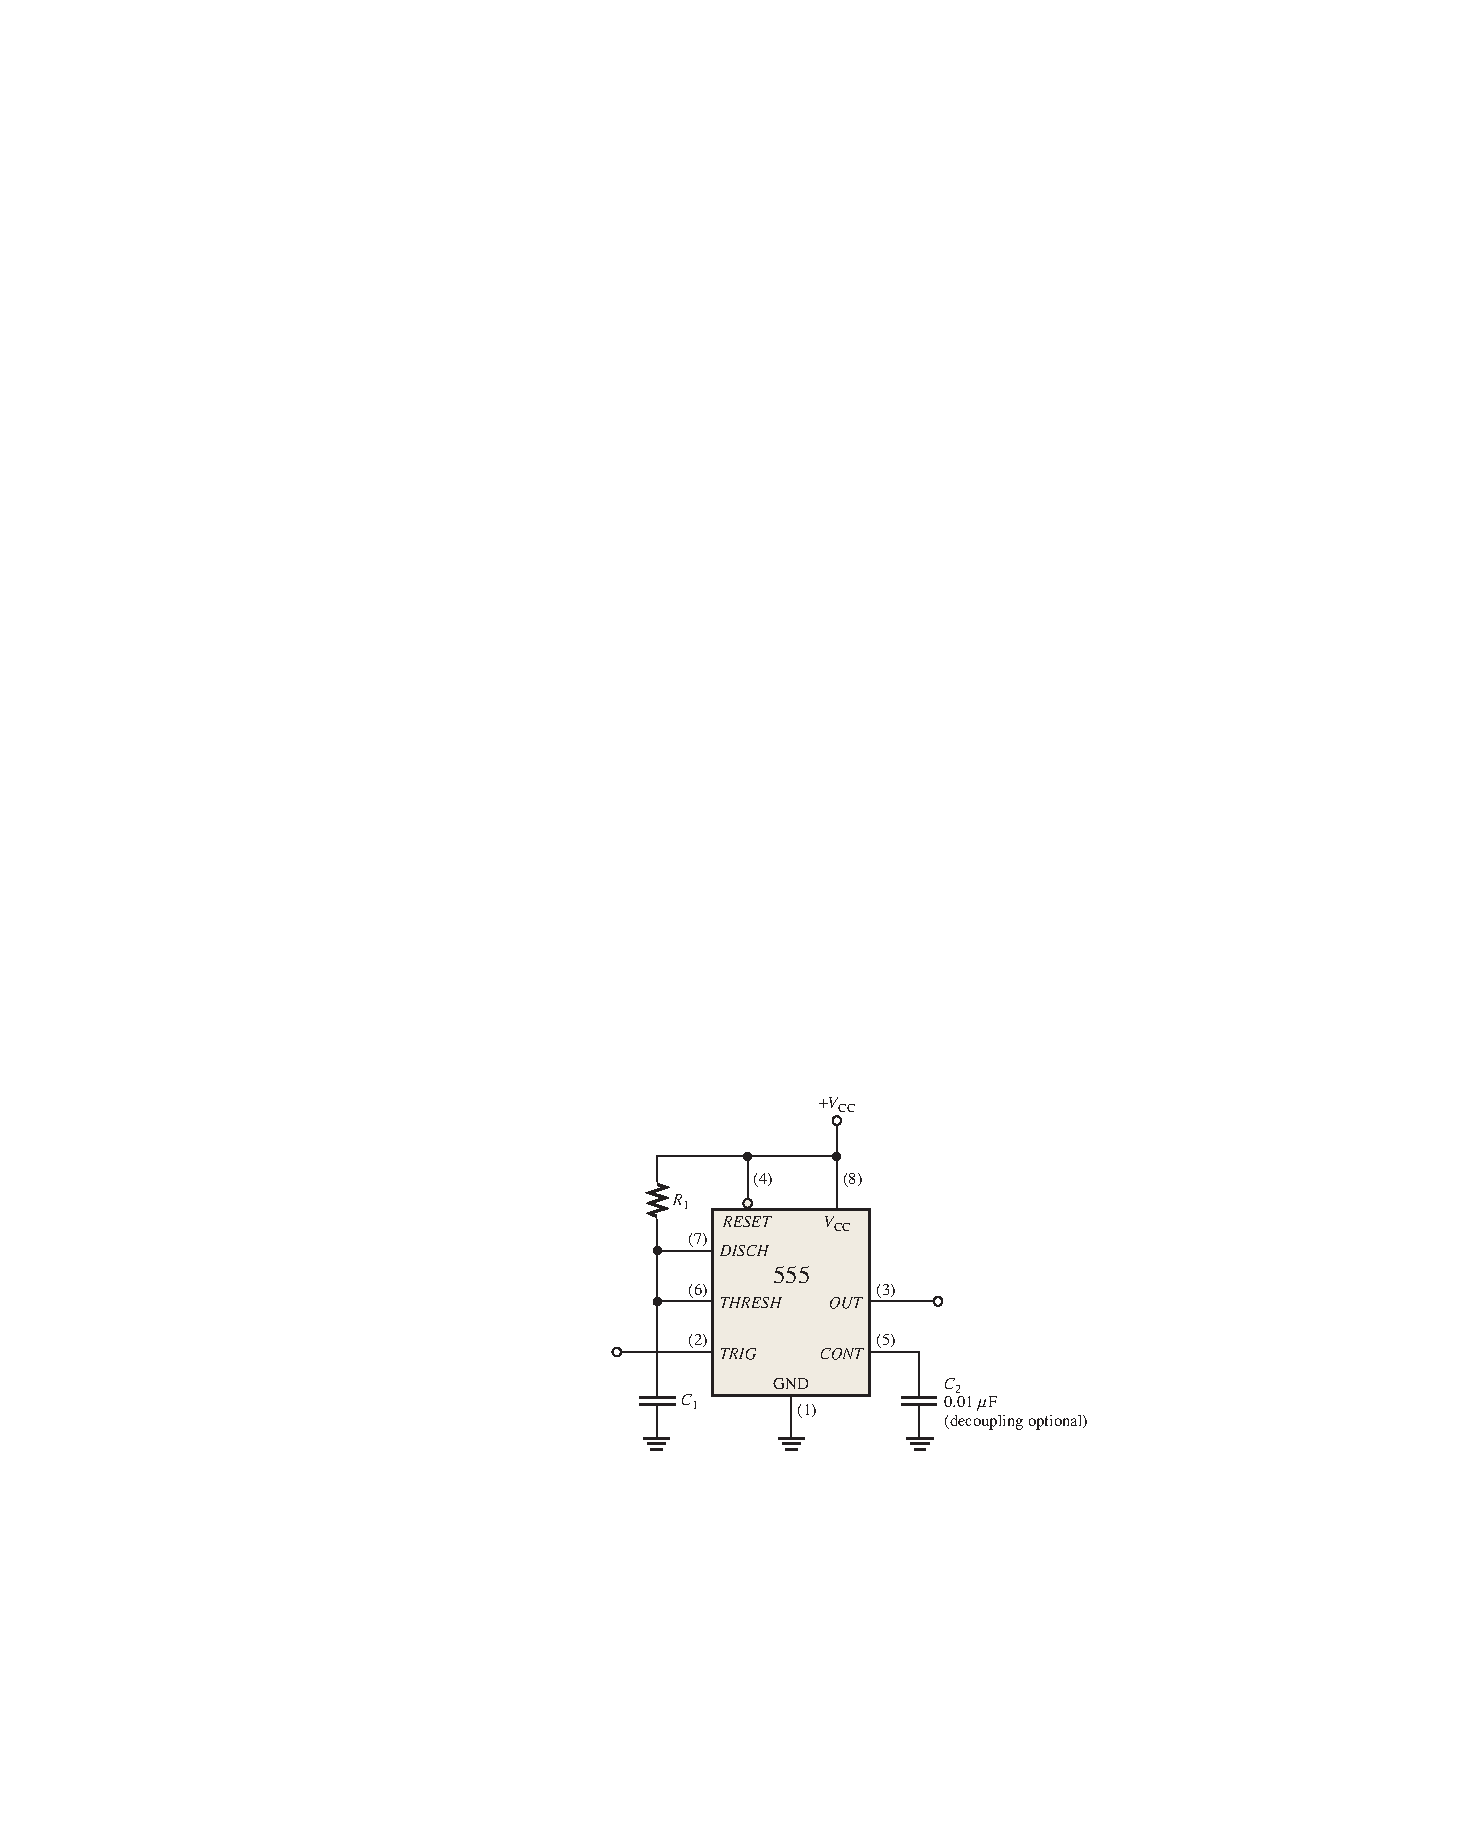
\includegraphics[scale = 1]{Graphics/Practice 2/GRAPHICS/555/GRAPHS/MODES/MONOSTABLE.pdf}
    \caption{555 timer connected as an monostable multivibrator (One-shot). ~\autocite{FLOYD}}
    \label{fig:MONOSTABLE}
\end{figure}

As per the other configuration, the duration of the pulse $\mathbf{t_{p}}$ or $\mathbf{t_{w}}$ can be determined by the next equation:

\begin{equation*}
    t_{p} = 1.1 \cdot R_1 \cdot C_1
\end{equation*}

For this configuration, the trigger is a NGP (Negative-going pulse). In the manufacturer's datasheet we can find a chart similar to the last one: \medskip

\begin{figure}[H]
    \centering
    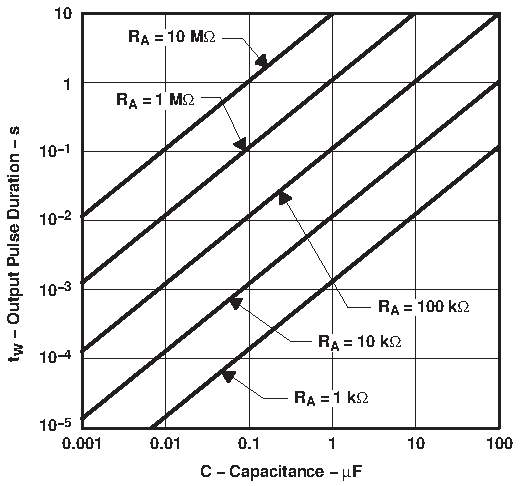
\includegraphics[scale = 0.8]{Graphics/Practice 2/GRAPHICS/555/GRAPHS/DATASHEETS/MONOSTABLE_FREQ.pdf}
    \caption{555 timer Monostable Frequency Chart. ~\autocite{555_DS}}
    \label{fig:MONOSTABLE_FREQ}
\end{figure}

\clearpage


\subsection{Exercise 1: 555 as Astable Multivibrator}

\textit{Design an astable multivibrator by using 555 timer with C = 10 nF, $R_1$ = 10 k$\Omega$ y $R_2$ = 10 k$\Omega$. Calculate theoretically the value of $t_H$ (high level semi period), T (period) and DC\% (duty cycle).}\medskip

\textit{Draw and simulate the circuit. Obtain the graphics of the outputs and between the pins of the capacitor. Measure the values of $t_H$ (high level semi period), T (period) and DC\% (duty cycle).}\bigskip

\textbf{\large Answer to Exercise 1:}\medskip

Using the equations listed in \ref{fig:ASTABLE_FREQ} and \ref{fig:DUTY}, obtaining what we are asked is rather simple:

\vspace{-.5cm}

\begin{align*}
    \mathbf{t_H} &= 0.693 \cdot (R_1 + R_2) \cdot C_1 = 0.693 \cdot (10k\Omega + 10k\Omega) \cdot 10\si\nano \text{F} = \mathbf{138.6 \, \textbf{\si\micro s}}
    \\
    \mathbf{t_L} &= 0.693 \cdot (R_2) \cdot C_1 = 0.693 \cdot (10k\Omega) \cdot 10\si\nano \text{F} = \mathbf{69.3 \, \textbf{\si\micro s}}
    \\
    \mathbf{T} &= t_L + t_H = \mathbf{207.9 \, \si\micro \text{s}}
    \\
    \mathbf{D} &= \frac{t_H}{t_H + t_L} \cdot 100= \frac{\mathbf{138.6 \, \si\micro \text{s}}}{\mathbf{138.6 \, \si\micro \text{s} + \mathbf{69.3 \, \textbf{\si\micro s}}}} \cdot 100 = \mathbf{66.6 \, \text{\%}}
\end{align*}\medskip

We are also asked to simulate the circuit. To do this we will make use of ISIS Proteus, as we have done in the past. 

\begin{figure}[H]
    \centering
    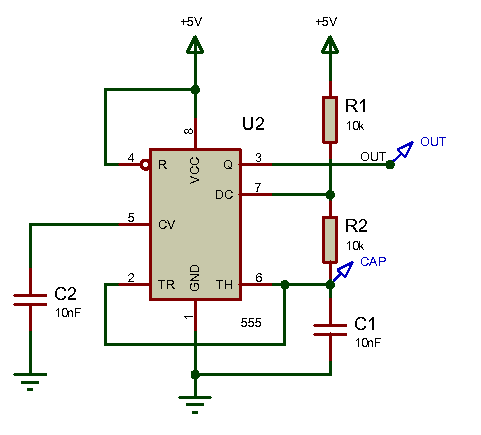
\includegraphics[scale = 1.1]{Graphics/Practice 2/GRAPHICS/555/GRAPHS/PROTEUS/ASSEMBLY/555_ASTABLE_10K_ASSEMBLY.PDF}
    \caption{Proteus assembly of the first subsection with $R_2 = 10k \Omega$.}
    \label{fig:555_ASTABLE_10K_ASSEMBLY}
\end{figure}

\clearpage

To check the output, we will employ the Analogue Analysis tool:

\begin{figure}[H]
    \centering
    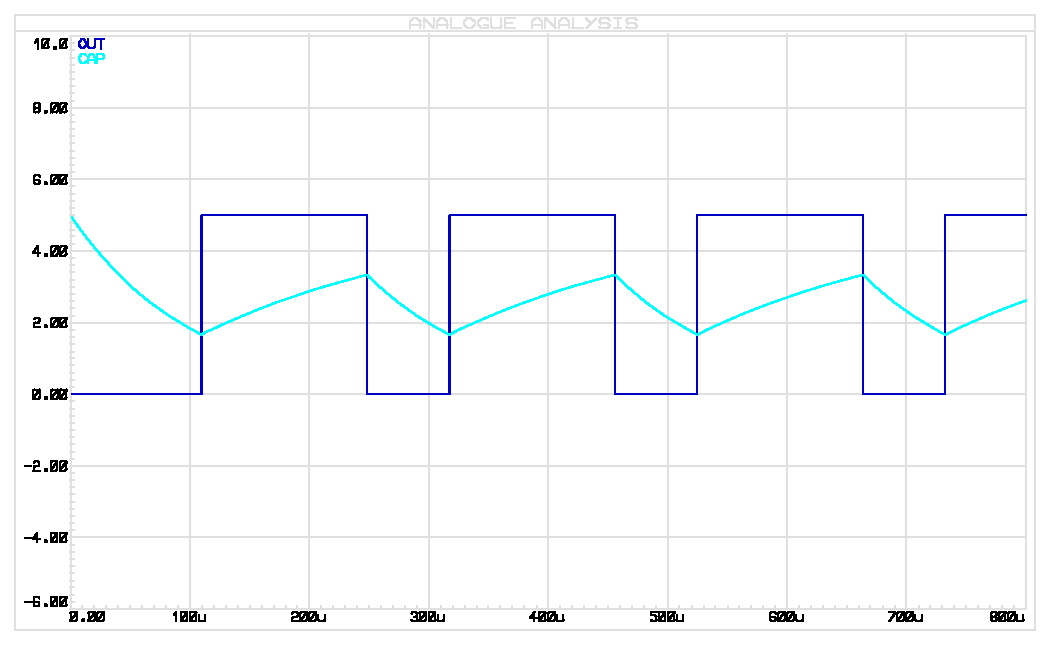
\includegraphics[scale = 0.75]{Graphics/Practice 2/GRAPHICS/555/GRAPHS/PROTEUS/ANALOGUE/555_ASTABLE_ANALOGUE_10K.PDF}
    \caption{Analogue Analysis of circuit with $R_2 = 10k \Omega$.}
    \label{fig:555_ASTABLE_ANALOGUE_10K}
\end{figure}


Using the cursors, we can measure the required parameters:

\begin{equation*}
    \mathbf{t_H} = \mathbf{207 \, \si\micro \text{s}} \quad
    \mathbf{t_L} = \mathbf{69 \, \si\micro \text{s}} \quad
    \mathbf{T} = \mathbf{207 \, \si\micro \text{s}} \quad
    \mathbf{D} =  \mathbf{66.6 \, \text{\%}}
\end{equation*}\medskip

As we can see, they match the calculations perfectly since proteus doesn't take into account the tolerances of the different components. The same simulation in NI Multisim yields vastly different results, due to its mathematical models of components being more accurate.\medskip

\clearpage

The exercise now asks us to change the value of $R_2$ to $100k\Omega$ and measure the same parameters. After following the same procedure, we obtain these results:

\begin{figure}[H]
    \centering
    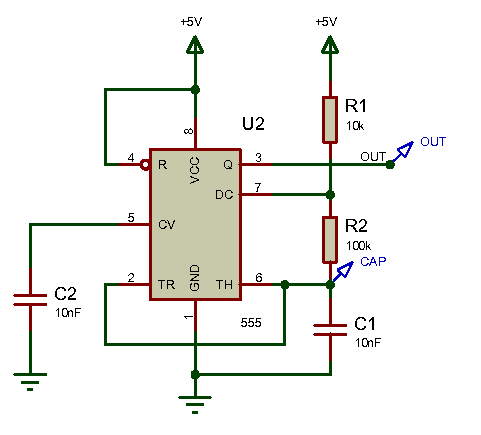
\includegraphics[scale = 1.1]{Graphics/Practice 2/GRAPHICS/555/GRAPHS/PROTEUS/ASSEMBLY/555_ASTABLE_100K_ASSEMBLY.PDF}
    \caption{Proteus assembly of the second subsection with $R_2 = 100k \Omega$.}
    \label{fig:555_ASTABLE_100K_ASSEMBLY}
\end{figure}

\begin{figure}[H]
    \centering
    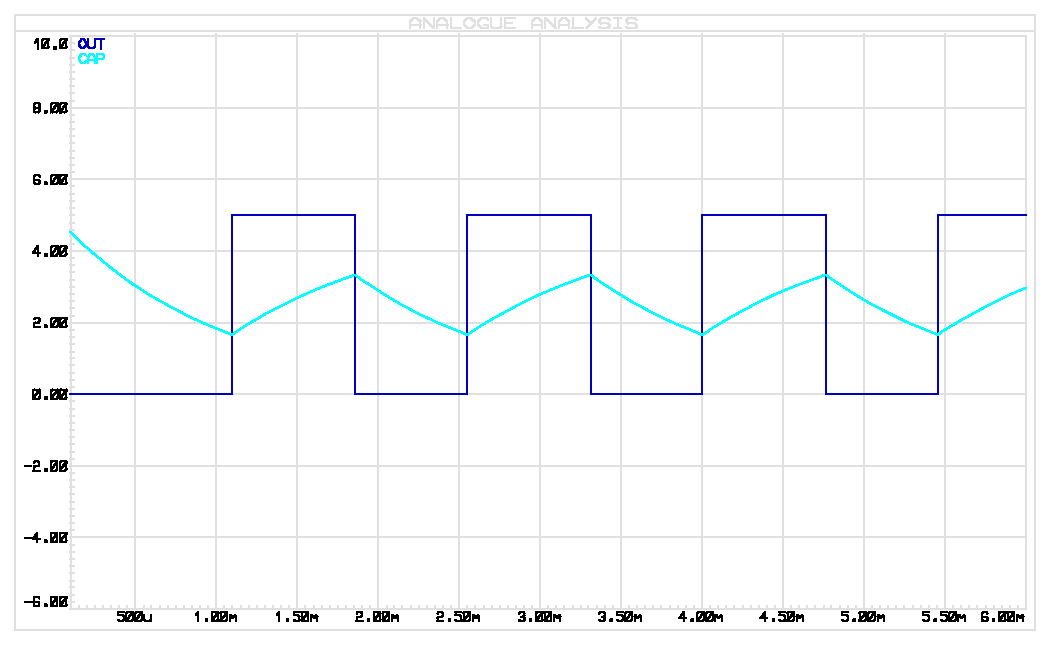
\includegraphics[scale = 0.75]{Graphics/Practice 2/GRAPHICS/555/GRAPHS/PROTEUS/ANALOGUE/555_ASTABLE_ANALOGUE_100K.PDF}
    \caption{Analogue Analysis of circuit with $R_2 = 100k \Omega$.}
    \label{fig:555_ASTABLE_ANALOGUE_100K}
\end{figure}

\vspace{-.4cm}

\begin{equation*}
    \mathbf{t_H} = \mathbf{762 \, \si\micro \text{s}} \quad
    \mathbf{t_L} = \mathbf{693 \, \si\micro \text{s}} \quad
    \mathbf{T} = \mathbf{1455 \, \si\micro \text{s}} \quad
    \mathbf{D} =  \mathbf{52.37 \, \text{\%}}
\end{equation*}
\clearpage


The exercise finally asks us to add a diode in parallel with $R_2$ and measure the same parameters. After following the same procedure, we obtain these results:

\begin{figure}[H]
    \centering
    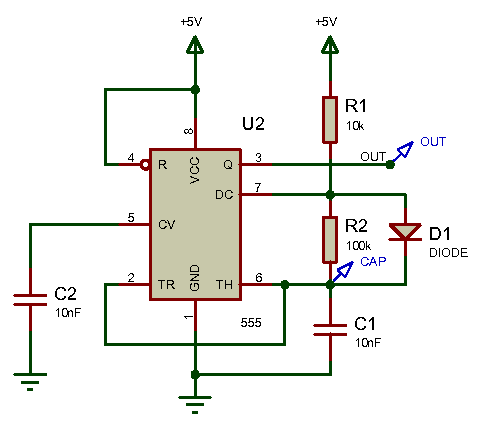
\includegraphics[scale = 1.1]{Graphics/Practice 2/GRAPHICS/555/GRAPHS/PROTEUS/ASSEMBLY/555_ASTABLE_100K_DIODE_ASSEMBLY.PDF}
    \caption{Proteus assembly of the third subsection with $R_2 = 100k \Omega$ and a diode in parallel.}
    \label{fig:555_100K_DIODE}
\end{figure}


\begin{figure}[H]
    \centering
    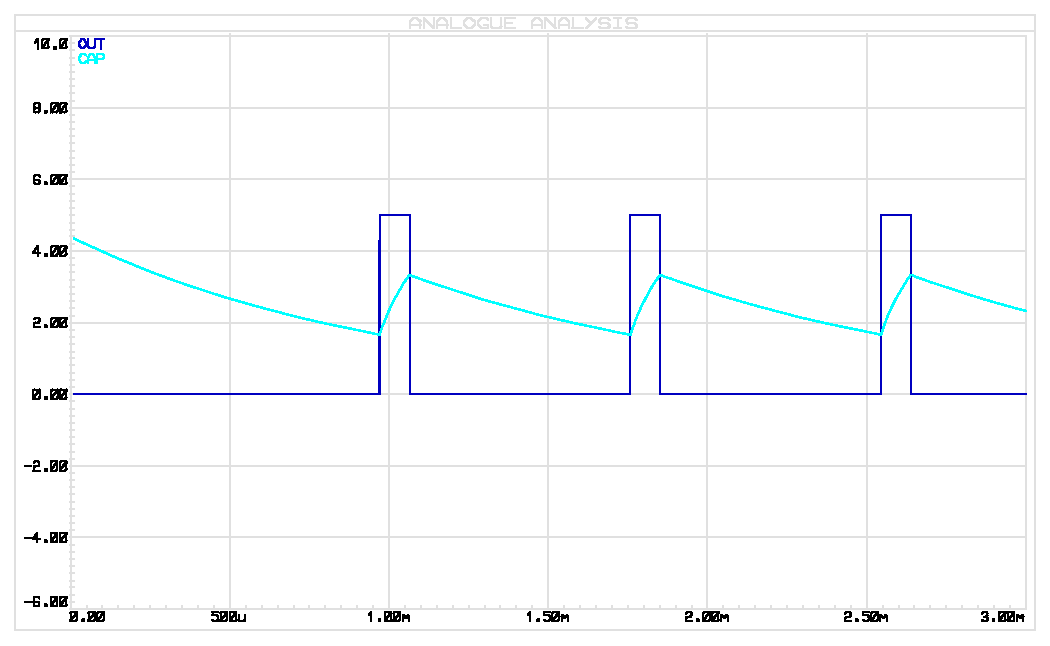
\includegraphics[scale = 0.8]{Graphics/Practice 2/GRAPHICS/555/GRAPHS/PROTEUS/ANALOGUE/555_ASTABLE_ANALOGUE_100K_DIODE.PDF}
    \caption{Analogue Analysis with $R_2 = 100k\Omega$ and Diode in parallel.}
    \label{fig:555_ANALOGUE_100K_DIODE}
\end{figure}

\vspace{-.4cm}

\begin{equation*}
    \mathbf{t_H} = \mathbf{98 \, \si\micro \text{s}} \quad
    \mathbf{t_L} = \mathbf{690 \, \si\micro \text{s}} \quad
    \mathbf{T} = \mathbf{788 \, \si\micro \text{s}} \quad
    \mathbf{D} =  \mathbf{12.44 \, \text{\%}} 
\end{equation*}


\subsection{Exercise 2: 555 as Monostable Multivibrator}

In this exercise we are asked to design a one-shot multivibrator (Figure \ref{fig:MONOSTABLE} )using a 555 timer, a 10 \si\micro F capacitor and a $100k\Omega$ resistor. As a reminder, the duration of the pulse of a 555 monostable can be obtained using this equation:

\begin{equation*}
    t_{p} = 1.1 \cdot R_1 \cdot C_1 = 1.1 \cdot 100k\Omega \cdot 10 \si\micro \text{F} = 1.10 \text{s}
\end{equation*}


\begin{figure}[H]
    \centering
    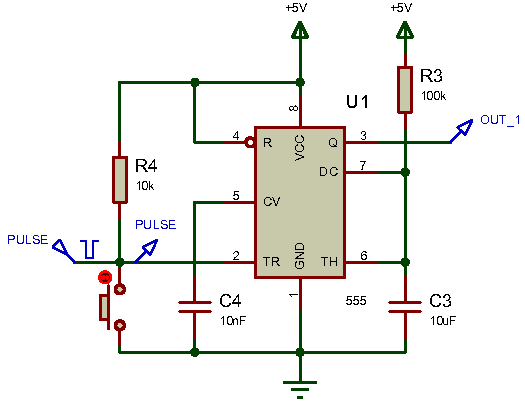
\includegraphics[scale = 1.045]{Graphics/Practice 2/GRAPHICS/555/GRAPHS/PROTEUS/ASSEMBLY/555_MONO_ASSEMBLY.PDF}
    \caption{Proteus assembly of a Monostable Multivibrator}
    \label{fig:555_MONO_ASSEMBLY}
\end{figure}


\begin{figure}[H]
    \centering
    
    \ifnum\value{ANIMATION}=1 {
        \animategraphics[controls,loop,scale=0.75]{1}{Graphics/Practice 2/GRAPHICS/ANIMATION/555/555_MONO_ANALOGUE_F}{0}{1}
    } 
    \else {
        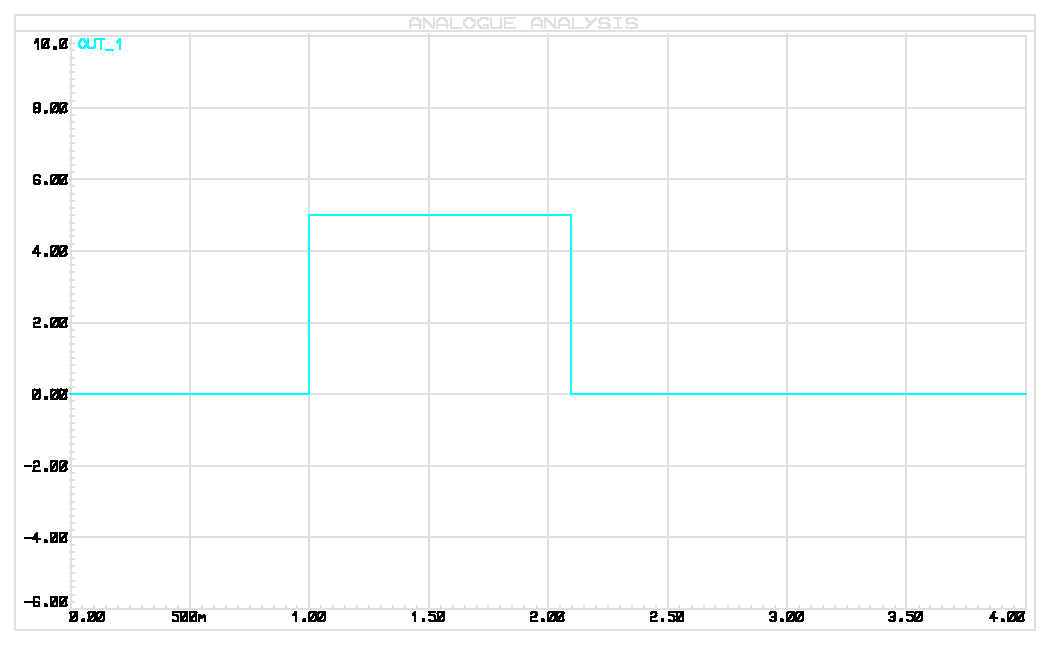
\includegraphics[scale=0.75]{Graphics/Practice 2/GRAPHICS/ANIMATION/555/555_MONO_ANALOGUE_F1.PDF}
    }\fi
    
    \caption{Analog Analysis of a Monostable Multivibrator.}
    \label{fig:555_MONO_ANALOGUE}
\end{figure}

\clearpage

